
This chapter presents the chosen case study, which serves as a stimulus for system design and demonstrates 
the practical application of the developed work. The chosen case study focuses on the \gls{crc} peripheral,
which is present in several microcontroller families, such as STM32 \cite{referenceManualRM0385} or Xilinx Zynq \cite{xilinx2014zynq} 
nevertheless, the VExpress\_gem5, which is a board introduced by gem5, does not have it.

The \gls{crc} was created in 1961 by William Wesley Peterson \cite{peterson1961cyclic}. As the name suggests, 
it utilizes systematic cyclic codes to encode messages by incorporating a fixed-length check value. In the end, his work
contributed significantly to simplifying and enhancing the detection of accidental errors/changes in communication 
networks. \gls{crc} uses a generator polynomial, which is known by the sender and receiver, and it is used to 
perform the calculation. There are different standards however, the most common ones are the CRC-8, CRC-12, CRC-16, 
CRC-32, and CRC-CCIT \cite{borrelli2001ieee}

Another application for the \gls{crc} is the storage integrity. Due to defective components or electromagnetic fields,
bits can change their value without notice. In the presented case study, this scenario will be explored, where 
the \gls{crc} peripheral is used to maintain a specific memory state and verify if there have been any changes. 
Furthermore, to showcase the advantages of the previously developed work, the application will perform other 
tasks simultaneously. 

\section{CRC peripheral} %Software development

As mentioned earlier in this dissertation, co-simulation involves the integration of multiple simulation tools from different
domains. Because of that, it is required to develop a system that can execute and communicate among them. The following picture
demonstrates how the different tools will communicate with each other.

\begin{figure}[H]
	\centering
 	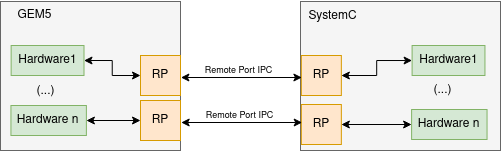
\includegraphics[width=0.8\linewidth]{Images/CoSimDesignSimplified.png}
 	\caption{Co-simulation design}
	 \label{fig_CoSimDesignSimplified}
\end{figure}

The communication will be done using a remote port \gls{ipc}. This should be created and connected before the beginning of the
simulation, in a way that transactions occur. Further, gem5 will use the \gls{uart} to communicate with the user by the terminal. 
This peripheral is already implemented, hence it only requires its initialization and configuration. The subsequent sections will delve into 
the detailed explanations of the \gls{crc} component. It's worth noting that the design process 
took significant reference from the STM32 microcontroller family's reference manual.


\subsection{SystemC}

The peripheral development was carried out using the SystemC tool. In this example, it will only simulate the \gls{crc} but, it has
the capability to simulate more than just one peripheral. For instance, picture a scenario where the workload also requires an \gls{adc}.
This peripheral is also not included in the VExpress\_gem5 board, so it would also require its implementation. For this reason, flexibility
is a requirement, and with this idea in mind, the subsequent design was developed.

\begin{figure}[H]
	\centering
	\begin{subfigure}{0.45\textwidth}
		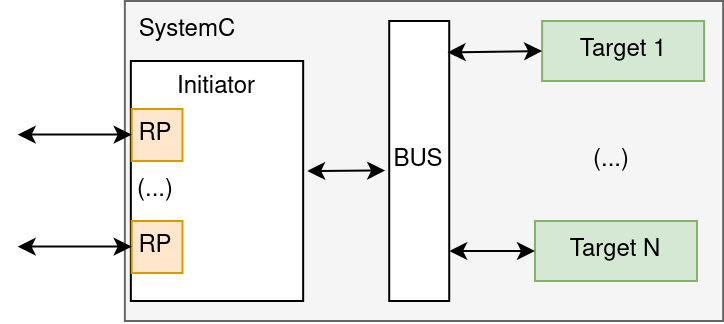
\includegraphics[width=\textwidth]{Images/SystemCdesign.png}
 		\caption{General SystemC design}
	 	\label{fig_SystemCdesign_geral}
	\end{subfigure}
	\hfill
	\begin{subfigure}{0.45\textwidth}
		\centering
		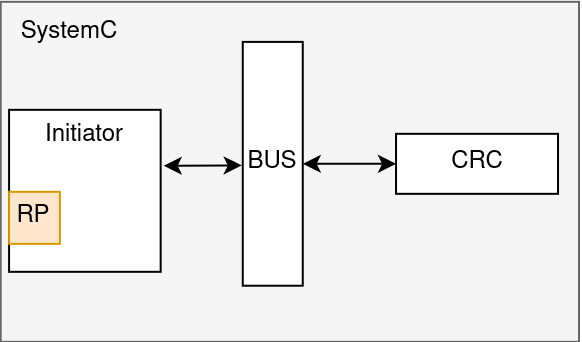
\includegraphics[width=\textwidth]{Images/SystemCdesign_CRC.png}
		\caption{SystemC design with CRC}
		\label{fig_SystemCdesign_CRC}
	\end{subfigure}
		
	\label{fig:SystemCsdesign}
\end{figure}


It is composed of three main components. The initiator, the bus, and the targets. Beginning with the first, it serves as the initial 
point of interaction for the tool, as it handles incoming frames received through the remote port. The remote port operates independently 
of the initiator, enabling asynchronous reception and transmission of bytes through the receiver and transmit buffers, respectively.
Additionally, it also performs an interpretation of the received trama and creates the \gls{tlm} transaction. It analyses various 
parameters such as the operation type, the desired target, and the memory region, among others, with the help of \gls{tlm} wrapper, 
which will presented in the \autoref{subsec::TLMwrapper}.

The bus is responsible for forwarding the \gls{tlm} transaction to the right target. Each target has a unique ID, that is attributed to it 
at the beginning of the simulation. Gem5's board is a 32-bit processor, meaning that each transaction is 32-bit in length. However, SystemC 
\gls{tlm} transactions can be 64-bit, leaving 32 bits unused. Before the transmission, the initiator uses these bytes to set the 
target\_ID, which will be utilized by the bus to identify the targets.

Lastly, the targets are the peripherals, that can be different from each other, as mentioned in the previous example. These receive the 
\gls{tlm} commands and act accordingly. Since in this dissertation, the focus will be the \gls{crc}, a single target will be implemented
thus, the \autoref{fig_SystemCdesign_geral} can be redefined to the \autoref{fig_SystemCdesign_CRC}. This will have the following
characteristics. 

\begin{itemize}
	\item Uses CRC-32 (Ethernet) polynomial: 0x4C11DB7
	\item Programmable CRC initial value
	\item Single input/output 32-bit data register
	\item CRC computation done in 4 clock cycles 
	\item General-purpose 8-bit register (can be used for temporary storage)
	\item Reversibility option on I/O data
\end{itemize}

\begin{figure}[]
	\centering
 	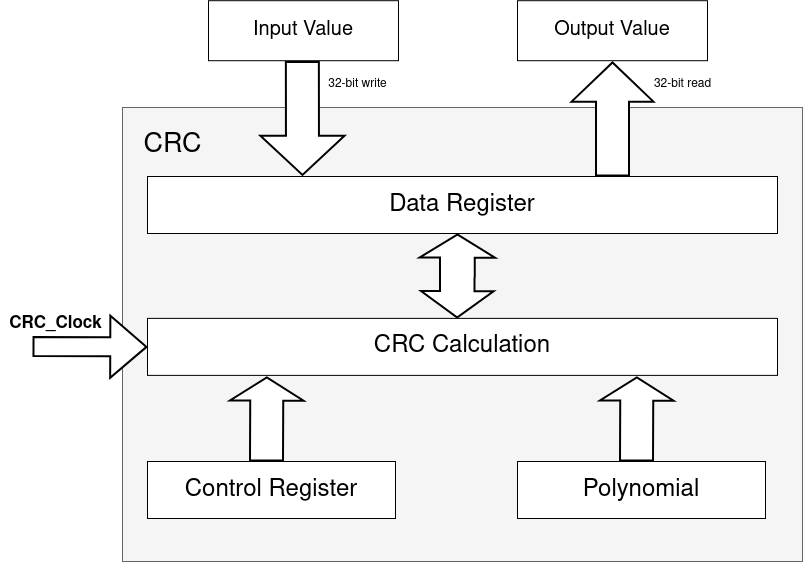
\includegraphics[width=0.6\linewidth]{Images/CrcBlockDiagram.png}
 	\caption{CRC block diagram}
	 \label{fig_CrcBlockDiagram}
\end{figure}

The peripheral will work as demonstrated in \autoref{fig_CrcBlockDiagram}. First of all, the user needs to write the input value 
in the data register (CRC\_DR). After four \gls*{crc} clock cycles, the correspondent \gls*{crc} value is fully calculated, and its
value is stored in the CRC\_DR. In this case, the \gls*{crc} frequency with be equal to the \gls*{cpu}. The data width must be 32-bit, 
hence whether the user needs a \gls*{crc} for five bytes, for example, two different computations will be needed. 

Moreover, the input and output data can be reversed, to manage the various endianness schemes. For the input data, the reverse operation 
is controlled by the REV\_IN[1:0] bits, and for the output data, the REV\_OUT bit is used. These, along with the reset bit used to 
reset the \gls*{crc}, are located in the control register (CRC\_CR). An example of a reverse operation can be found on \autoref{tab:CRC_REV}.

\begin{table}[!htb]
    \caption{Reverse operation}
    \begin{minipage}{.5\linewidth}
      \centering
      \subcaption{Input}
		\resizebox{\textwidth}{!}{%
		\begin{tabular}{lllll}
		\cline{1-4}
		\multicolumn{1}{|l|}{\cellcolor[HTML]{C0C0C0}{\color[HTML]{000000} REV\_IN[1:0]}} & \multicolumn{1}{l|}{\cellcolor[HTML]{C0C0C0}{\color[HTML]{000000} Input}} & \multicolumn{1}{l|}{\cellcolor[HTML]{C0C0C0}{\color[HTML]{000000} Reverse Action}} & \multicolumn{1}{l|}{\cellcolor[HTML]{C0C0C0}{\color[HTML]{000000} Reverse Input}} &  \\ \cline{1-4}
		\multicolumn{1}{|l|}{0 0} & \multicolumn{1}{l|}{0x1A2B3C4D} & \multicolumn{1}{l|}{Not affected} & \multicolumn{1}{l|}{0x1A2B3C4D} &  \\ \cline{1-4}
		\multicolumn{1}{|l|}{0 1} & \multicolumn{1}{l|}{0x1A2B3C4D} & \multicolumn{1}{l|}{Bit-reversal done by byte} & \multicolumn{1}{l|}{0x58D43CB2} &  \\ \cline{1-4}
		\multicolumn{1}{|l|}{1 0} & \multicolumn{1}{l|}{0x1A2B3C4D} & \multicolumn{1}{l|}{Bit-reversal done by half-word} & \multicolumn{1}{l|}{0xD458B23C} &  \\ \cline{1-4}
		\multicolumn{1}{|l|}{1 1} & \multicolumn{1}{l|}{0x1A2B3C4D} & \multicolumn{1}{l|}{Bit-reversal done by word} & \multicolumn{1}{l|}{0xB23CD458} &  \\ \cline{1-4}
		&  &  &  & 
		\end{tabular}%
        }
        \label{tab:CRC_REV_IN}
    \end{minipage}%
    \begin{minipage}{.5\linewidth}
        \centering
        \subcaption{Output}
		\resizebox{\textwidth}{!}{%
		\begin{tabular}{lllll}
		\cline{1-4}
		\multicolumn{1}{|l|}{\cellcolor[HTML]{C0C0C0}{\color[HTML]{000000} REV\_OUT}} & \multicolumn{1}{l|}{\cellcolor[HTML]{C0C0C0}{\color[HTML]{000000} Output}} & \multicolumn{1}{l|}{\cellcolor[HTML]{C0C0C0}{\color[HTML]{000000} Reverse Action}} & \multicolumn{1}{l|}{\cellcolor[HTML]{C0C0C0}{\color[HTML]{000000} Reverse Output}} &  \\ \cline{1-4}
		\multicolumn{1}{|l|}{0} & \multicolumn{1}{l|}{0x11223344} & \multicolumn{1}{l|}{Not affected} & \multicolumn{1}{l|}{0x11223344} &  \\ \cline{1-4}
		\multicolumn{1}{|l|}{1} & \multicolumn{1}{l|}{0x11223344} & \multicolumn{1}{l|}{Bit-reversal done by word} & \multicolumn{1}{l|}{0x22CC4488} &  \\ \cline{1-4}
		 &  &  &  & 
		\end{tabular}%
        }   
        \label{tab:CRC_REV_OUT}
    \end{minipage}
	\label{tab:CRC_REV} 
\end{table}

By default, the polynomial coefficients are defined by 0x4C11DB7 nevertheless, it can be fully programmable through the CRC\_POL register.
It is important to mention that modifications in this register when a \gls*{crc} computation is ongoing are not permitted, as it would 
compromise the output value. To conclude the available registers, are missing the CRC\_INIT and CRC\_IDR, which are used to initialize 
the \gls*{crc} calculator in the reset, and to hold a temporary 8-bit value related to \gls*{crc} calculation, respectively. 

Summing up, the \autoref{fig_CRC_write} and \autoref{fig_CRC_read} demonstrate how the peripheral will behave depending on the defined settings and desired 
operation. Before any execution, offset/size out-of-bounds, and permissions are verified to maintain the peripheral's integrity. The 
functionality of these parameters will be explained further. 

\begin{figure}[]
	\centering
 	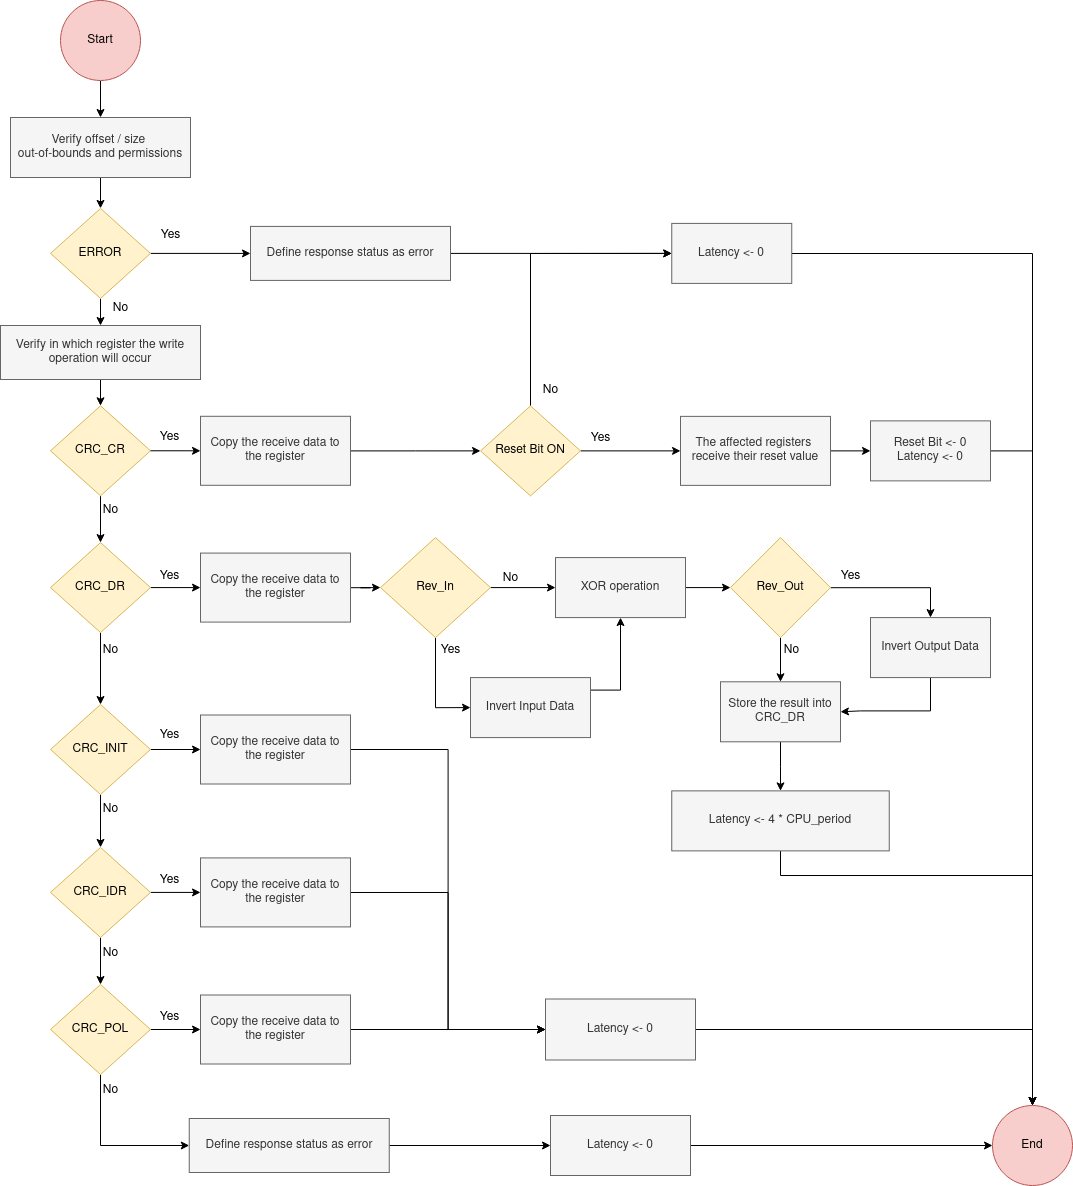
\includegraphics[width=0.6\linewidth]{Images/CRC_write.png}
 	\caption{CRC write operation}
	 \label{fig_CRC_write}
\end{figure}

\begin{figure}[]
	\centering
 	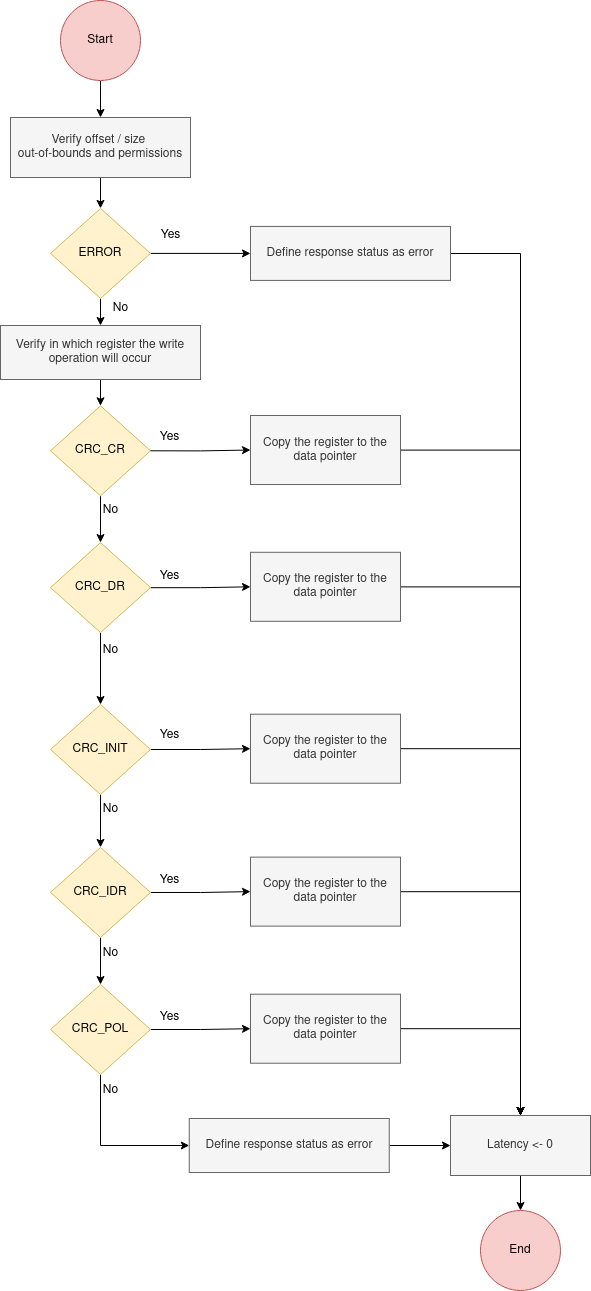
\includegraphics[width=0.6\linewidth]{Images/CRC_read.png}  %ROTATE TO HORIZONTAL
 	\caption{CRC read operation}
	 \label{fig_CRC_read}
\end{figure}


\subsection{Gem5}

Going into the gem5 domain, 

The VExpress\_gem5 board, which is introduced by gem5, does not have the understudy peripheral implemented thus, it was 
needed to reserve its memory space. The figure 

%CRC e considerado como um off chip peripheral
%Falar sobre de e necessario para assumir como um perifierico para a co-sim
%Necessario dizer ao gem5 que crc é um perifirico (armv7, adicionar ao realview)
%mostrar como foi implementado 

\subsection{TLM wrapper}
\label{subsec::TLMwrapper}

%Falar sobre este wrapper - O que é, porque existe(Porque o systemC e gem5 precisao de um "tradutor")
%Falar sobre a comunicação, do RP - feito com um socket
%Falar sobre a trama, playload e assim

\subsection{Application interface}

%Falar sobre o modulo CRC_SC
%Que funções tem, com aquele digrama de funcoes bonito
%Como existe com a biloteca HAL da STM

\section{Application simulation using gem5}

%Falar sobre as configurações da placa do vexpress
%Em que portas as coissas vao ficar connectadas
%perifericos que se vao utilizar

\begin{figure}[H]
	\centering
 	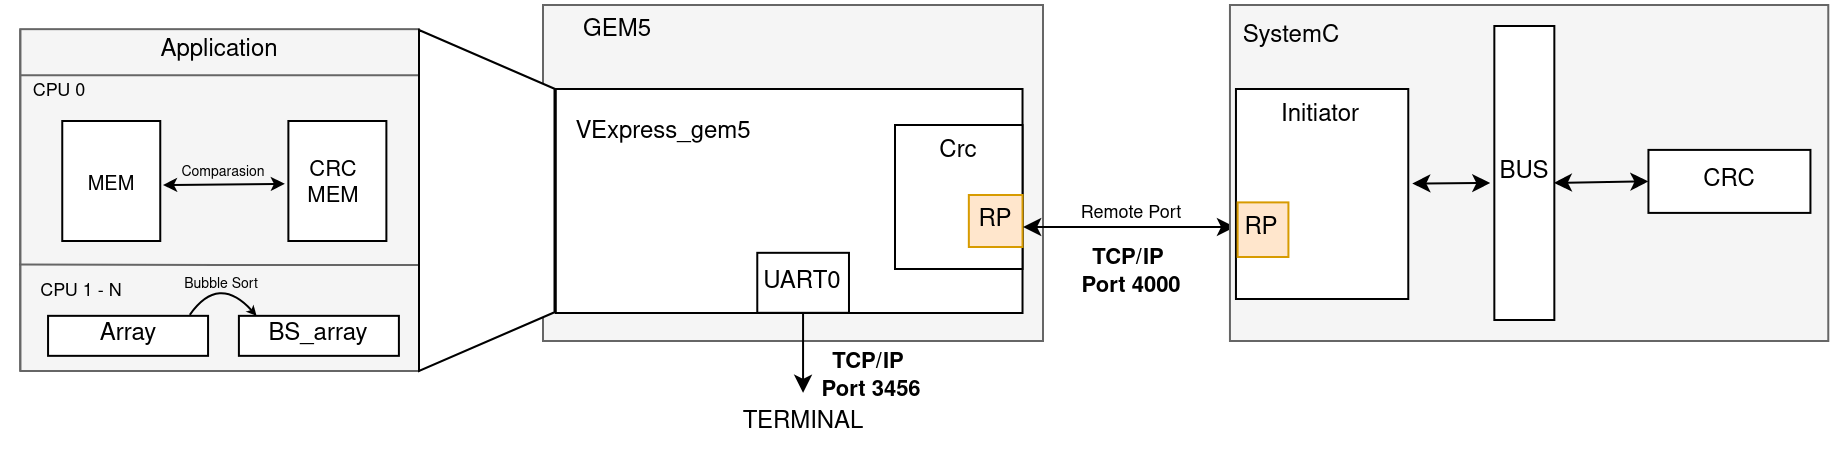
\includegraphics[width=0.9\linewidth]{Images/CoSimDesign.png}
 	\caption{Co-simulation design}
	 \label{fig_CoSimDesign}
\end{figure}

\subsection{CRC peripheral validation} 

%Mostrar como esta desenhado a aplicacao para validar o CRC

From the application point of view, the system will execute 2 distinct jobs. \gls{cpu}0 will be responsible for 
performing the memory integrity checks, while the remaining ones will execute a bubble sort algorithm. 



\begin{figure}[]
	\centering
 	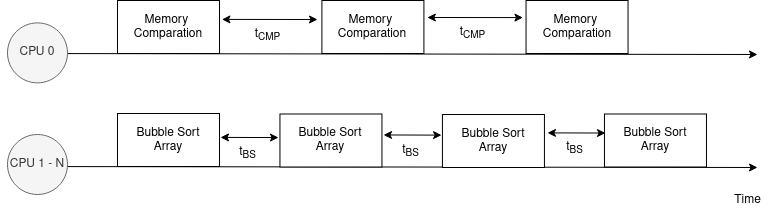
\includegraphics[width=0.7\linewidth]{Images/AppTimeDiagram.png}
 	\caption{Application execution timely diagram}
	 \label{fig_AppTimeDiagram}
\end{figure}


\section{Memory integrity}

%Entrar aqui no tema do proposito do CRC
%Mostrar que está a funcionar

\subsection{Fault Modeling}

%Mostrar como é que vai ser injetada a falha na memoria
%Mostrar que o sistema reage a falha

\section{Results}

%Aqui comparar os resultados com o meu algoritmo e sem ele
%Verificarar se houve algum melhoramento

